\newpage
\section*{MÉTODOS}
\addcontentsline{toc}{section}{MÉTODOS}
\par\refstepcounter{section}
\subsection{Campos de fuerza basados en conocimiento}
\par
Los potenciales de fuerza media utilizados y derivados en este trabajo parte del supuesto de que las fuerzas encontradas en sistemas moleculares grandes son excesivamente complejas, por lo tanto la única fuente de información confiable son estructuras resueltas en su estado nativo y en equilibrio. 
Si la extracción de información es exitosa, el campo de fuerza será capaz de determinar correctamente si un motivo en una molécula es nativo o no. 
Esta es la llamada aproximación deductiva o \textit{knowledge-based} de un potencial de fuerza 
media. (\cite{Sippl1993})
\par
Un potencial de fuerza media parte de la ley inversa de Boltzmann:
\begin{equation}
E_{ijkl} = -kT\log(f_{ijkl}) + kT\log Z \label{boltz1}
\end{equation}
La función de energía E\textsubscript{ijkl} es el llamado potencial de fuerza media. 
La variable \textit{f} es la frecuencia relativa de un cierto estado al fijar las variables i, j, k, l en 
los sistemas observados en nuestra base de datos. 
\textit{Z} representa la función de partición y no puede ser calculada experimentalmente, y se le da el 
valor de 1 (\cite{Sippl1993}). 
La ecuación \eqref{boltz1}  entonces toma la forma:
\begin{equation}
E_{ijkl} = -kT\log(f_{ijkl}) \label{boltz2}
\end{equation}
\par
Pero para utilizar exitosamente la ley inversa de Boltzmann es necesario también definir un sistema de referencia apropiado. 
Este se obtiene promediando un set elegido de variables del sistema, como por ejemplo k y l.
Esto nos permite extraer una característica energética general de los sistemas, las cuáles también se definen como un potencial de energía:
\begin{equation}
E_{kl} = -kT\log(f_{kl}) \label{boltzref}
\end{equation}
\par
Con esto, ahora podemos obtener el valor neto del potencial de fuerza media:
\begin{equation}
\Delta E^{ij}_{kl} = E^{ij}_{kl} - E_{kl} = -kT\log \left( \frac{f^{ij}_{kl}}{f_{kl}} \right)
\end{equation}
\par
En el contexto de este trabajo, nuestras variables \textit{i} y \textit{j} indican el tipo de interacción entre dos átomos (en el caso de los potenciales SASA, solo se usa la variable \textit{i}), mientras que \textit{k} y \textit{l} indican distancia en la secuencia de residuos y el \textit{bin} de la variable geométrica a analizar, que puede ser la distancia, BSASA o SASA.
Se aplica también un factor de corrección para números bajos de observaciones en la base de datos, sugerido en \cite{Sippl1990}. 
Así, cuando en función de \textit{l} la ecuación final toma la forma:
\begin{equation}
\Delta E^{ij}_{k}(l) = RT\log \left[1 + M_{ijk}\sigma\right] - RT\log \left[ 1 + M_{ijk}\sigma \frac{f^{ij}_{k}(l)}{f_{k}(l)} \right] \label{finalboltz}
\end{equation}
Donde \textit{M\textsubscript{ijk}} corresponde al número de observaciones de interacciones del par al nivel de separación \textit{k}, y $\sigma$ al peso que se le da a cada observación. 
En este trabajo se utilizó $\sigma$ = 1/50. (\cite{Sippl1990,Melo1997})


\subsection{Determinación de tipos atómicos}
\par
Para los potenciales en proteínas, se utilizaron 40 tipos atómicos compartidos para los 20 aminoácidos.
Esto es debido a que existen 98 tipos atómicos no equivalentes en total, lo que resultaría en una base de datos con muy pocos datos para cada par de interacciones (\cite{Melo1997}).
Las definiciones se pueden ver en la Tabla \ref{table:atomprotdef}.
%tabla tipos
\newpage
\cleardoublepage
%\addcontentsline{lot}{table}{Definición de tipos atómicos para proteínas}
\begin{table}[!htp]
\begin{tabular}{ p{40pt} p{380pt} }
  \hline
  Tipo atómico & Lista de átomos \\
  \hline
  1 & \Ca\ para todos los aminoácidos excepto Glicina \\
  2 & \Ca\ Glicina \\
  3 & N para todos los aminoácidos excepto Prolina \\
  4 & C para todos los aminoácidos \\
  5 & O para todos los aminoácidos \\
  6 & Ala-\Cb, Ile-\Cgii, Ile-\Cd, Leu-\Cdi, Leu-\Cdii, Thr-\Cg, Val-\Cgi, Val-\Cgii \\
  7 & Ile-\Cb, Leu-\Cg, Val-\Cb \\
  8 & Arg-\Cb, Arg-\Cg, Asn-\Cb, Asp-\Cb, Gln-\Cb, Gln-\Cg, Glu-\Cb, Glu-\Cg, His-\Cb, Ile-\Cgi, Leu-\Cb, Lys-\Cb, Lys-\Cg, Lys-\Cd, Met-\Cb, Phe-\Cb, Pro-\Cb, Pro-\Cg, Trp-\Cb, Tyr-\Cb \\
  9 & Met-S\textsubscript{\text{\textdelta}} \\
 10 & Pro-N \\
 11 & Phe-\Cg, Trp-\Cdii, Tyr-\Cg \\
 12 & Phe-\Cdi, Phe-\Cdii, Phe-\Cei, Phe\Ceii, Phe-\Cz, Trp-\Ceiii, Trp-\Cz, Trp-\Cziii, Trp-\Cetaii, Tyr-\Cdi, Tyr-\Cdii, Tyr-\Cei, Tyr-\Ceii \\
 13 & Trp-\Cg \\
 14 & Trp-\Ceii \\
 15 & Ser-\Cb \\
 16 & Ser-O\textsubscript{\text{\textgamma}}, Thr-O\textsubscript{\text{\textgamma}} \\
 17 & Thr-\Cb \\
 18 & Asn-N\textsubscript{\text{\textdelta}2}, Gln-N\textsubscript{\text{\textepsilon}2} \\
 19 & Cys-S\textsubscript{\text{\textgamma}} \\
 20 & Lys-N\textsubscript{\text{\textzeta}} \\
 21 & Arg-\Cz \\
 22 & Arg-N\textsubscript{\text{\texteta}1}, Arg-N\textsubscript{\text{\texteta}2} \\
 23 & His-\Cg \\
 24 & His-\Cdii, Trp-\Cdi \\
 25 & His-N\textsubscript{\text{\textepsilon}2} \\
 26 & His-\Cei \\
 27 & Asp-\Cg, Glu-\Cd \\
 28 & Asp-O\textsubscript{\text{\textdelta}1}, Asp-O\textsubscript{\text{\textdelta}2}, Glu-O\textsubscript{\text{\textepsilon}1}, Glu-O\textsubscript{\text{\textepsilon}2} \\
 29 & Cys-\Cb, Met-\Cg \\
 30 & Met-\Ce \\
 31 & Tyr-\Cz \\
 32 & Pro-\Cd \\
 33 & Asn-\Cg, Gln-\Cd \\
 34 & Asn-O\textsubscript{\text{\textdelta}1}, Gln-O\textsubscript{\text{\textepsilon}1} \\
 35 & Lys-\Ce \\
 36 & Arg-N\textsubscript{\text{\textepsilon}} \\
 37 & Arg-\Cd \\
 38 & His-N\textsubscript{\text{\textdelta}1} \\
 39 & Trp-N\textsubscript{\text{\textepsilon}1} \\
 40 & Tyr-O\textsubscript{\text{\texteta}} \\
 \hline
\end{tabular}
\caption[Definiciones de átomos para proteínas]{Definiciones de átomos pesados utilizadas para potenciales en proteínas. Átomos del tipo 10 son convertidos al tipo 3 si son el primer residuo de una cadena proteíca.}
\label{table:atomprotdef}
\end{table}
%fin tabla tipos
\newpage
\clearpage
\par
En el caso de los potenciales para ADN y ARN, se utilizaron 23 tipos atómicos distintos descritos por \cite{Capriotti2011} para moléculas de ARN. A estos se agregaron dos tipos más, 24 y 25, correspondientes a los carbonos C5 y C7 (nombres IUPAC) del nucleótido timina.
Estas definiciones están en la Tabla \ref{table:atomnadef}.
%comienzo tabla nucleótidos
\newpage
\cleardoublepage
\begin{table}[!htp]
\begin{tabular}{p{40pt} p{380pt}}
  \hline \\
  Tipo atómico & Lista de átomos (nombres IUPAC) \\
  \hline \\
  1 & OP1, OP2, OP3 para todos los nucleótidos \\
  2 & P para todos los nucleótidos \\
  3 & O5' para todos los nucleótidos \\
  4 & C5' para todos los nucleótidos \\
  5 & C5', C3', C2' para todos los nucleótidos \\
  6 & O2', O3' terminales \\
  7 & C1' para todos los nucleótidos \\
  8 & O4' para todos los nucleótidos \\
  9 & N1 pirimidinas; N9 purinas \\
 10 & C8 purinas \\
 11 & N3, N7 en purinas; N1 en A; N3 en \\
 12 & C5 purinas \\
 13 & C4 purinas \\
 14 & C2 en A \\
 15 & C6 en A; C4 en C \\
 16 & N6 en A; N4 en C; N2 en G \\
 17 & C2 en G \\
 18 & C6 en G; C4 en U,T \\
 19 & O2 pirimidinas; O6 en G; O4 en U,T \\
 20 & C2 pirimidinas \\
 21 & C6 pirimidinas \\
 22 & C6 pirimidinas \\
 23 & N1 en G; N3 en U,T \\
 24 & C5 en T \\
 25 & C7 en T \\
 \hline
\end{tabular}
\caption[Definiciones de átomos para ADN y ARN]{Definiciones de átomos pesados utilizadas para potenciales en ARN y ADN. 
Se consideran tanto nucleótidos como deoxinucleótidos.}
\label{table:atomnadef}
\end{table}
%fin tabla nucleotidos
\newpage
\clearpage
\subsection{Derivación de potenciales basados en distancias y conteos de átomos}
\subsubsection{Derivación de potenciales basados en distancias}
\par
La derivación de los potenciales se hizo utilizando un programa escrito en C++, dada la gran cantidad de datos a procesar.
Se utilizaron los mismos parámetros de derivación utilizados en \cite{Melo1998} para los potenciales en proteínas, por lo que solo se consideran interacciones entre átomos a 7 \si{\angstrom} de distancia y separados por un mínimo de 13 residuos si los átomos pertenecen a una misma cadena.

\par
Para los potenciales en ARN y ADN, se utilizan los parámetros similares a los utilizados en \cite{Capriotti2011}, donde se usan 6 funciones distintas. Todas estas funciones consideran interacciones a 7 \si{\angstrom} de distancia en vez de 20 \si{\angstrom}.
Las primeras 5 funciones solo consideran como interacciones átomos que están exactamente a 1, 2, 3, 4 y 5 residuos de distancia más cualquier interacción en otra cadena. 
La última función solo considera interacciones a 6 o más residuos de distancia.
Las distancias entre los átomos están discretizadas en 35 \textit{bins} uniformes de 0.2 \si{\angstrom}, paso necesario para obtener datos de frecuencia.
Los pasos descritos en el algoritmo \ref{alg:deralgo1} son los mínimos necesarios para la generación del potencial. 
Las variables \textit{Radius, Lmin, Lmax, Nbins y Sigma} corresponden respectivamente a la distancia máxima de interacción, la distancia mínima entre residuos de una misma cadena que se considera como interacción, la distancia máxima entre residuos de una misma cadena que se considera como interacción, la cantidad de \textit{bins} en que se divide el rango de distancia, y el valor de corrección $\sigma$.

\begin{algorithm}[H]
\caption{Pasos para la derivación de un potencial a partir de una lista de archivos PDB}\label{alg:deralgo1}
\begin{algorithmic}[0]
\Procedure{GeneratePotential}{}
\State $ \text{matrix2D } Mij $ \Comment{Tabla de conteo de interacciones de tipo I con tipo J}
\State $ \text{matrix3D } Fij $ \Comment{Tablas de frecuencia de interacciones para cada intervalo de distancia}
\State $ \text{matrix1D } Fxx $ \Comment{Lista de frecuencia de interacciones en cierto intervalo de distancia}

\State $ \text{list } pdblist \gets \text{GetPDBs}(argv1) $ \Comment{Carga estructuras PDB desde lista de archivos en disco}
\For {$ \textit{pdbstruct} \text{ in } \textit{PDBlist} $}
\State $ \text{CalculateInteractions}(pdbstruct,Radius,Lmin,Lmax) $ \Comment{Calcula los contactos entre átomos y sus distancias}
\EndFor
\State $ \text{DDCalculateIntFreq}(PDBlist,Fix,Fxx,Mij,Nbins) $ \Comment{Calcula todas las tablas necesarias para la derivación del potencial}
\State $ \text{WritePotential}(Fij,Fxx,Mij,Nbins,Sigma) $ \Comment{Escribe el potencial creado a disco}
\EndProcedure
\end{algorithmic}
\end{algorithm}

\par
En la figura \ref{fig:energy1} se pueden observar algunos de los potenciales generados utilizando el método descrito para moléculas de proteína. 
El archivo en disco contiene la información de estas funciones en un formato de texto, el que se utiliza posteriormente para la evaluación de la energia en otras estructuras.
En la figura \ref{fig:mij} se observa la matriz de conteo de interacciones (triángulo superior), cuyos datos se usan para el factor de corrección $\sigma$ usado en la Ecuación \ref{finalboltz}.
\clearpage
\begin{figure}[p]
\centering
\begin{subfigure}{.8\textwidth}
\centering
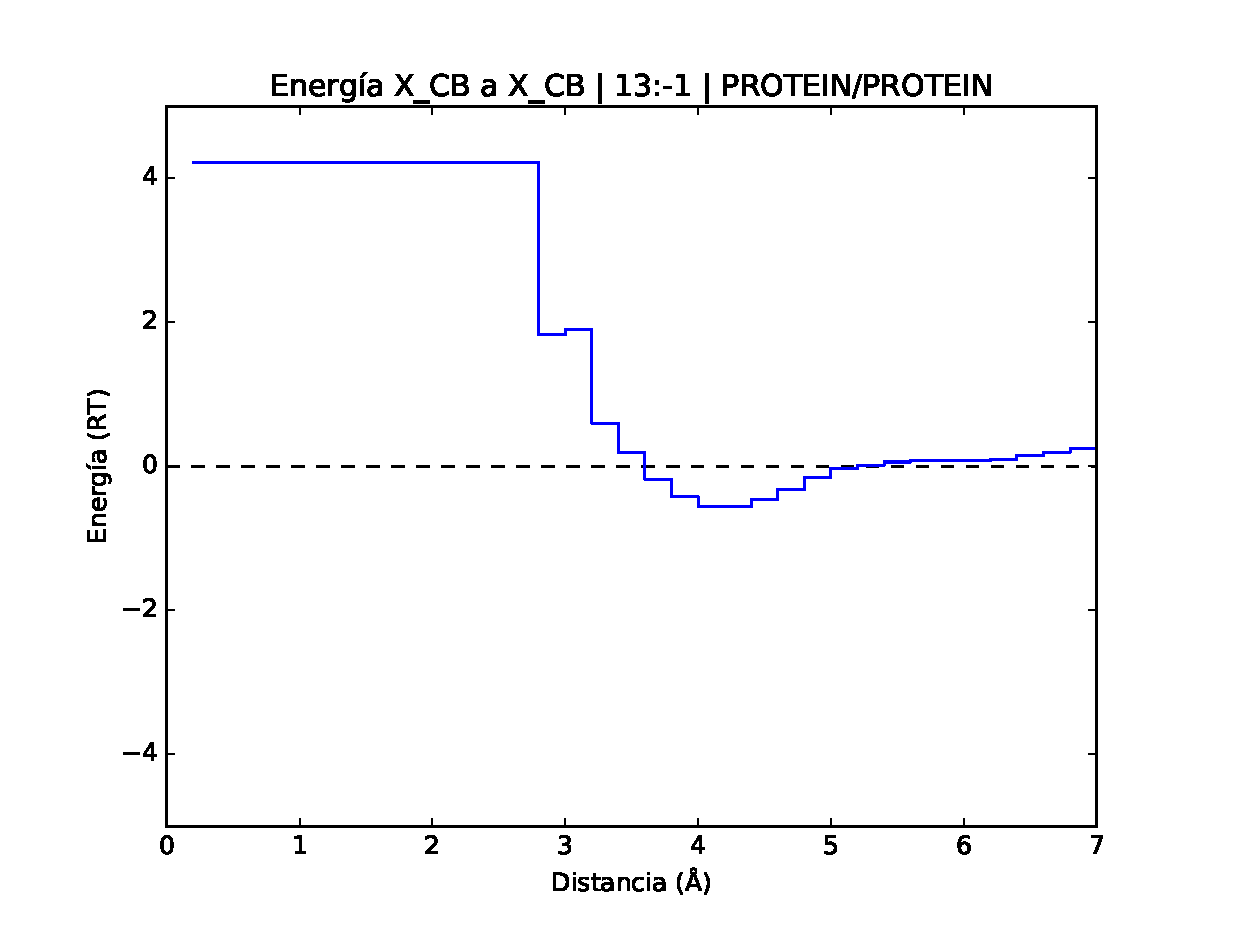
\includegraphics[width=\textwidth]{figures/prot_pot/eps_graphs/cb2cb.eps}
\caption{}
\end{subfigure}

\begin{subfigure}{.8\textwidth}
\centering
\includegraphics[width=\textwidth]{figures/prot_pot/eps_graphs/sh2sh.eps}
\caption{}
\end{subfigure}
\caption[Ejemplos de funciones de energía en proteínas]{Gráficos de las funciones de energía utilizadas en proteínas. 
En (a) se observa la energía (unidades RT) en función de la distancia en \si{\angstrom} para los carbonos beta de todos los aminoácidos. 
En (b) se tiene la función de energia para los átomos de azufre de císteina, representando los puentes disulfuro.}
\label{fig:energy1}
\end{figure}

\begin{figure}[p]
\includegraphics[width=\textwidth]{figures/prot_pot/mij.png}
\caption[Cálculo de $\sigma$]{Matriz de conteo de interacciones para los potenciales en proteína, o \textit{Mij}. 
Solo se usa el triángulo superior de esta estructura, ya que no se considera el orden de las interacciones. 
Conteos están en escala logaritmíca para facilitar la visualización.}
\label{fig:mij}
\end{figure}

\cleardoublepage
\subsubsection{Derivación de potenciales basados en conteos de átomos}
\par
Estos potenciales están basados en el conteo de la cantidad de centros atómicos en cierto rango de distancia.
Como no dependen de interacciones entre pares de átomos, se debe modificar la Ecuación \ref{finalboltz}:
\begin{equation}
\Delta E^{i}_{k}(l) = RT\log \left[1 + M_{ik}\sigma\right] - RT\log \left[ 1 + M_{ik}\sigma \frac{f^{i}_{k}(l)}{f_{rel}} \right] \label{surfboltz}
\end{equation}



\subsection{Cálculo de la superficie accesible al solvente de una molécula}
\par
Para el cálculo de la superfície accesible al solvente o SASA se utilizó el llamado algoritmo de Shrake y Rupley (\cite{Shrake1973}), descrito en Algoritmo \ref{shrkrply1}. Este consiste generar para cada átomo de una estructura una nube de puntos con forma esférica que estan a una distancia de radio de Van der Waals más el radio de una molécula de una molécula de agua del centro del átomo. 
Cada punto representa un área equivalente al área de una esfera con el radio descrito anteriormente dividido por el número de puntos. Al eliminar los puntos que se encuentran en el interior del volumen de las nubes de puntos de otros átomos, es posible obtener la superficie accesible al contar los puntos restantes y multiplicarlos por el valor de superficie que representan.
\par
La nube de puntos debe tener todos sus puntos lo más equidistantes posible en el plano esférico para que el cálculo de superficie no tenga sesgos debido a la distribución de los puntos.



\begin{algorithm}[H]
\caption{Pasos para la obtención del SASA de una estructura }\label{alg:deralgo1}
\begin{algorithmic}[0]
\Procedure{CalculateSASA}{}
\State $ \text{pdbstruct } Mij $ \Comment{Estructura PDB}
\State $ \text{list unitsphere } Fij $ \Comment{Lista de puntos 3D equidistantes en la superficie de una esfera unitaria}
\State $ \text{matrix1D } Fxx $ \Comment{Lista de frecuencia de interacciones en cierto intervalo de distancia}

\State $ \text{list } pdblist \gets \text{GetPDBs}(argv1) $ \Comment{Carga estructuras PDB desde lista de archivos en disco}
\For {$ \textit{pdbstruct} \text{ in } \textit{PDBlist} $}
\State $ \text{CalculateInteractions}(pdbstruct,Radius,Lmin,Lmax) $ \Comment{Calcula los contactos entre átomos y sus distancias}
\EndFor
\State $ \text{DDCalculateIntFreq}(PDBlist,Fix,Fxx,Mij,Nbins) $ \Comment{Calcula todas las tablas necesarias para la derivación del potencial}
\State $ \text{WritePotential}(Fij,Fxx,Mij,Nbins,Sigma) $ \Comment{Escribe el potencial creado a disco}
\EndProcedure
\end{algorithmic}
\end{algorithm}


\subsection{Cálculo de las subsuperfícies de interacción}
\par
\subsection{Derivación de potenciales basados en BSA}
\par
\subsection{Derivación de potenciales basados en SASA}
\par
\subsection{Cálculo del IP (\textit{Information Product})}
